\section{Flat Obstacles}
Some non-lethal obstacles are defined by a flat cost, such as the interaction areas of \citet{fraichard:anthronav} or the perimeter of the parking lot in \citet{likhachev:costmaps}. In this trivial case, the marginal cost is
\begin{equation}
   \displaystyle
   f(x, y) = \left\{
     \begin{array}{lr}
       A & : (x,y) \in Q\\
       0 & : (x,y) \notin Q
     \end{array}
   \right.
\end{equation}
Each move traversing a cell in the obstacle set has a costs of $A$. 

\begin{figure}[b]
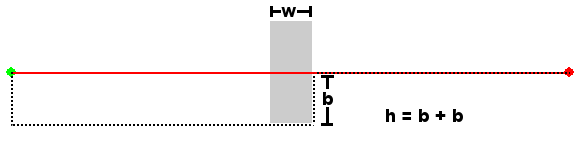
\includegraphics[width=\columnwidth]{graphix/Constant.png}
\caption{Two Paths with a Flat obstacle - The direct path (solid line) travels straight through the obstacle. The other path avoids the obstacle, but needs to travel an additional distance $d$.}
\label{fig:constant}
\end{figure}

We will plan a path from $(n, 0)$ to $(-n, 0)$, computing the cost by summing the baseline cost-per-move $P$ and the marginal cost-per-move $f$ over each move.

\begin{equation}
C(p) = \sum\limits_{(x,y)\in p} P + f(x, y)
\end{equation}

For a rectangular step obstacle placed at the origin with dimensions $w\times h$, there are essentially two feasible paths, illustrated in Figure \ref{fig:constant}. The direct path costs
\begin{equation}
C(p_1) = 2nP + wA
\end{equation}

The best path around the obstacle costs

\begin{equation}
C(p_2) = (2n + h)P.
\end{equation}

The direct path is cheaper when the aspect ratio of the obstacle  is less than the ratio of costs:

\begin{equation}
\frac{w}{h} < \frac{P}{A}.
\end{equation}

This result is intuitive. If an obstacle is thin (small $w$) or the distance around the obstacle is quite large ($h$ is high), or going through the obstacle incurs a very small cost (low $A$), walk through the obstacle. 

To achieve the desired behavior, we can model the size and set the cost accordingly. This relationship can be adjusted accordingly for flat valued obstacles of different shapes. 




